\begin{figure*}[t!]
    \centering
    \begin{subfigure}[b]{0.22\linewidth}
        \centering
        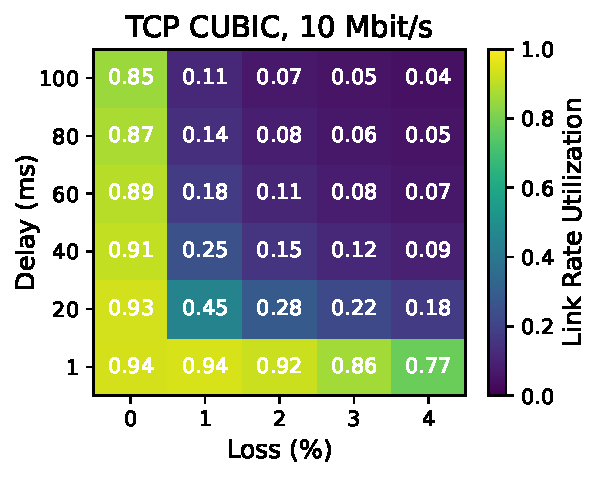
\includegraphics[width=\linewidth,trim={0 0 2cm 0.7cm},clip]
         {splitting-paper/figures/heatmaps/heatmap_tcp_cubic_10mbps.pdf}
        \captionsetup{skip=4pt}
        \caption{TCP CUBIC.}
        \label{fig:2d-heatmap:cubic-10}
    \end{subfigure}
    \begin{subfigure}[b]{0.22\linewidth}
        \centering
        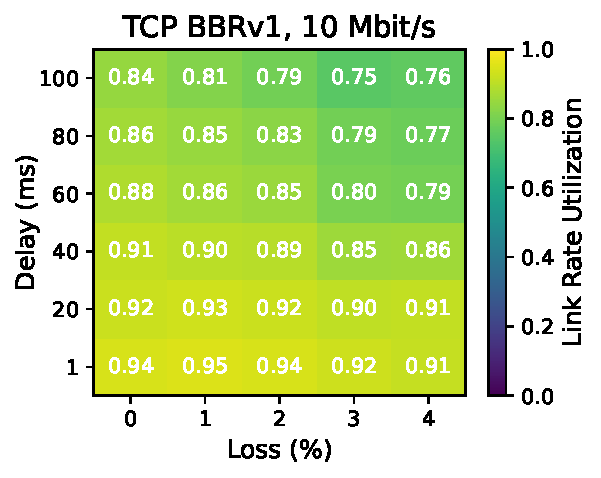
\includegraphics[width=\linewidth,trim={0 0 2cm 0.7cm},clip]
         {splitting-paper/figures/heatmaps/heatmap_tcp_bbr1_10mbps.pdf}
        \captionsetup{skip=4pt}
        \caption{TCP BBRv1.}
        \label{fig:2d-heatmap:bbr1-10}
    \end{subfigure}
    \begin{subfigure}[b]{0.22\linewidth}
        \centering
        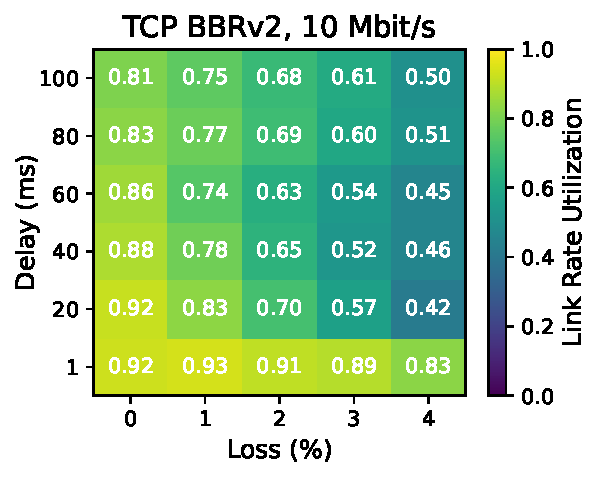
\includegraphics[width=\linewidth,trim={0 0 2cm 0.7cm},clip]
         {splitting-paper/figures/heatmaps/heatmap_tcp_bbr2_10mbps.pdf}
        \captionsetup{skip=4pt}
        \caption{TCP BBRv2.}
        \label{fig:2d-heatmap:bbr2-10}
    \end{subfigure}
    \begin{subfigure}[b]{0.22\linewidth}
        \centering
        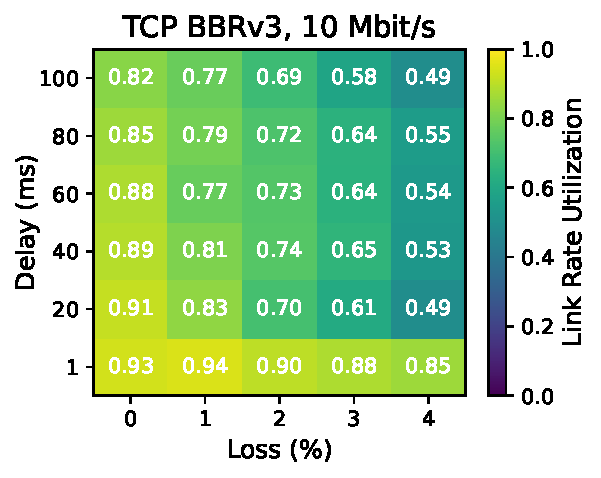
\includegraphics[width=\linewidth,trim={0 0 2cm 0.7cm},clip]
         {splitting-paper/figures/heatmaps/heatmap_tcp_bbr3_10mbps.pdf}
        \captionsetup{skip=4pt}
        \caption{TCP BBRv3.}
        \label{fig:2d-heatmap:bbr3-10}
    \end{subfigure}
    \begin{subfigure}[b]{1cm}
        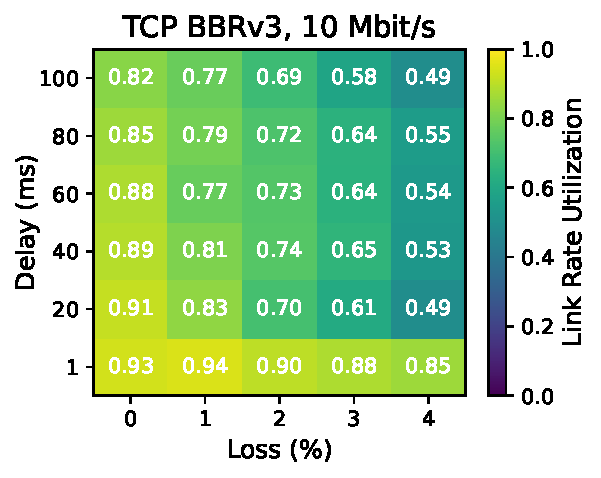
\includegraphics[width=1cm,trim={8cm 0 0 0},clip]
         {splitting-paper/figures/heatmaps/heatmap_tcp_bbr3_10mbps.pdf}
    \end{subfigure}
    \caption{The link rate utilization calculated as the ratio of achieved
     goodput to link rate for various TCP CCAs in an emulated network path, at
     various loss rates and one-way delays, at 10 Mbit/s. CUBIC is the
     most sensitive to loss and delay, while BBRv1 is the most aggressive and
     achieves the highest utilizations; BBRv2 and BBRv3 are more sensitive to
     loss than BBRv1 and utilization starts to suffer (left to right). CCAs
     tend to achieve lower utilizations, though higher absolute goodputs, as
     the link rate increases (\Cref{sec:appendix}). Median of $n=20$ trials.}
    \label{fig:2d-heatmap}
\end{figure*}
